\subsection{Ajuster le faisceau laser}
\begin{enumerate}
   \item Si présent, retirer le \textit{beam dump}~(voir figure~\ref{fig:beam-dump}) placé à la sortie du RegA.
        \begin{figure}[H]
        \centering
        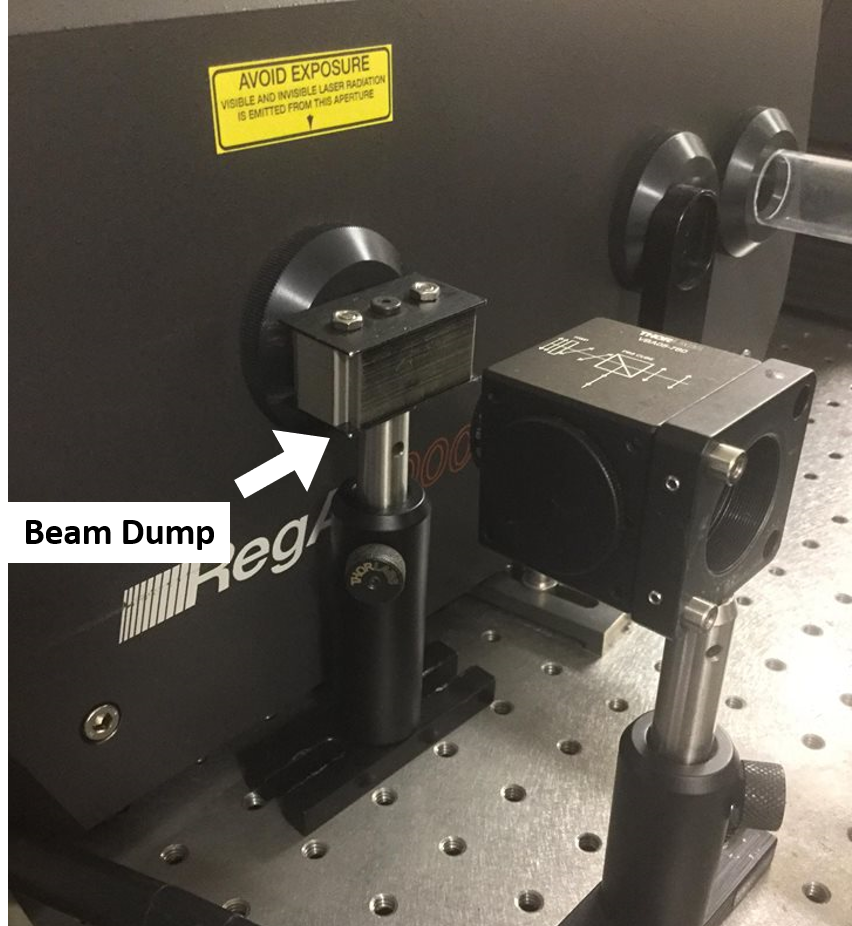
\includegraphics[height=6cm]{beam-dump.png}
        \caption{Beam Dump}
        \label{fig:beam-dump}
        \end{figure}
    \item Tel que montré à la figure~\ref{fig:puissance}, placer le \textit{capteur du puissancemètre} après le \textit{diviseur de puissance}.
        \begin{figure}[H]
        \centering
        \includegraphics[width=15cm]{puissance.png}
        \caption{Mesure de la puissance du laser}
        \label{fig:puissance}
        \end{figure}
    \item Tourner l'\textit{anneau} du \textit{diviseur de puissance} afin d'obtenir une puissance d'environ 750-900~W. Attention:~Le faisceau laser qui sort du RegA ne doit pas revenir sur lui-même. Par conséquent, le \textit{diviseur de puissance} ne doit pas être parfaitement à 90~degrés de la sortie du RegA mais plutôt légèrement tourné (environ 3~degrés) pour que la réflexion soit dirigée ailleurs. On peut le tourner après avoir desserré la vis située sur son pied.
    \item Retirer le \textit{capteur} du trajet optique.
        \begin{figure}[H]
        \centering
        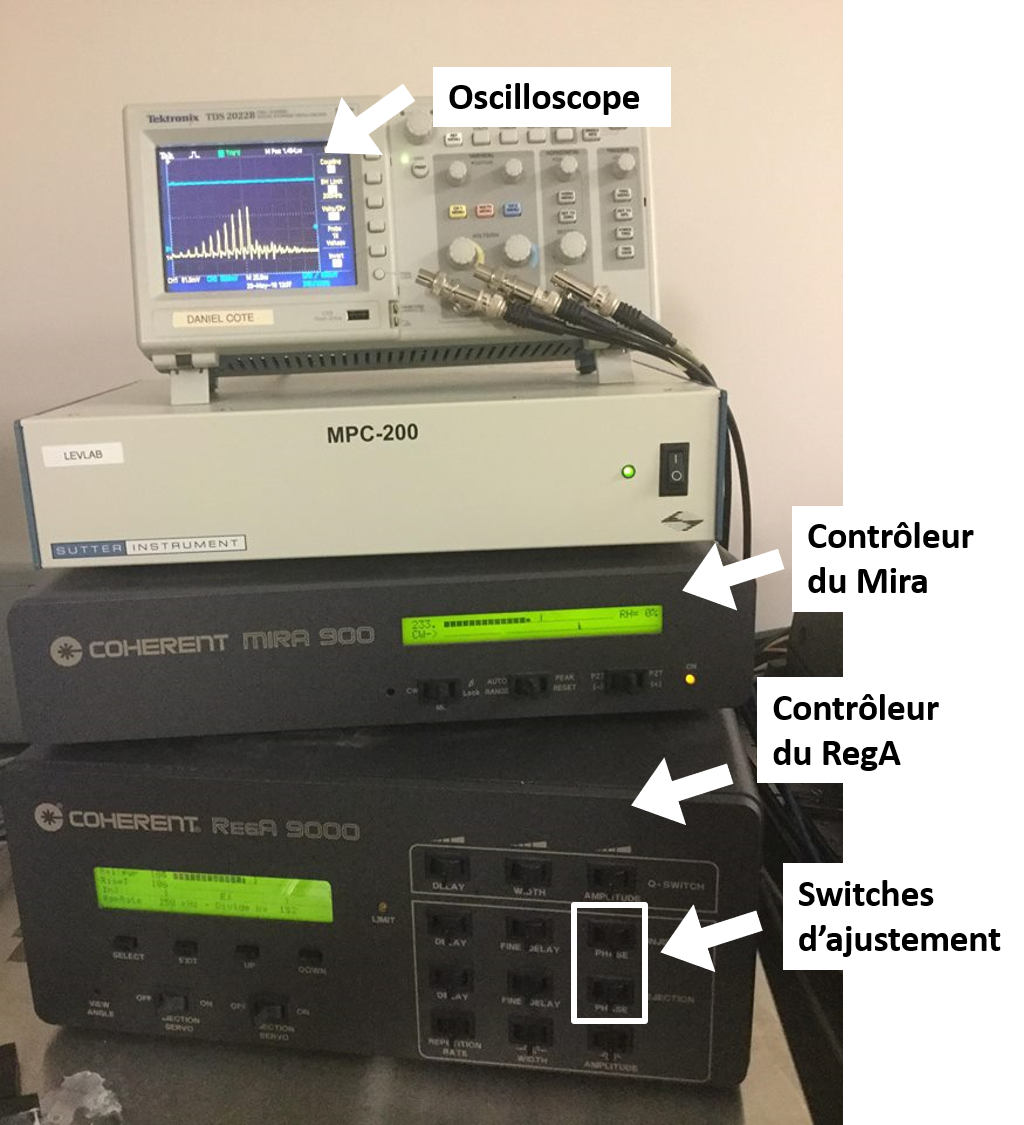
\includegraphics[width=10cm]{controleurs.png}
        \caption{Contrôleurs}
        \label{fig:controleurs}
        \end{figure}
    \item Sur le \textit{contrôleur du Mira} (voir figure~\ref{fig:controleurs}), mettre la bascule de gauche sur \textit{ML}.
    \item Sur le \textit{contrôleur du Mira}, vérifier que le taux d'humidité (RH) est entre 0\% et 5\%. Si non, augmenter le flux d'azote fourni au système, i.e.:
        \begin{figure}[H]
        \centering
        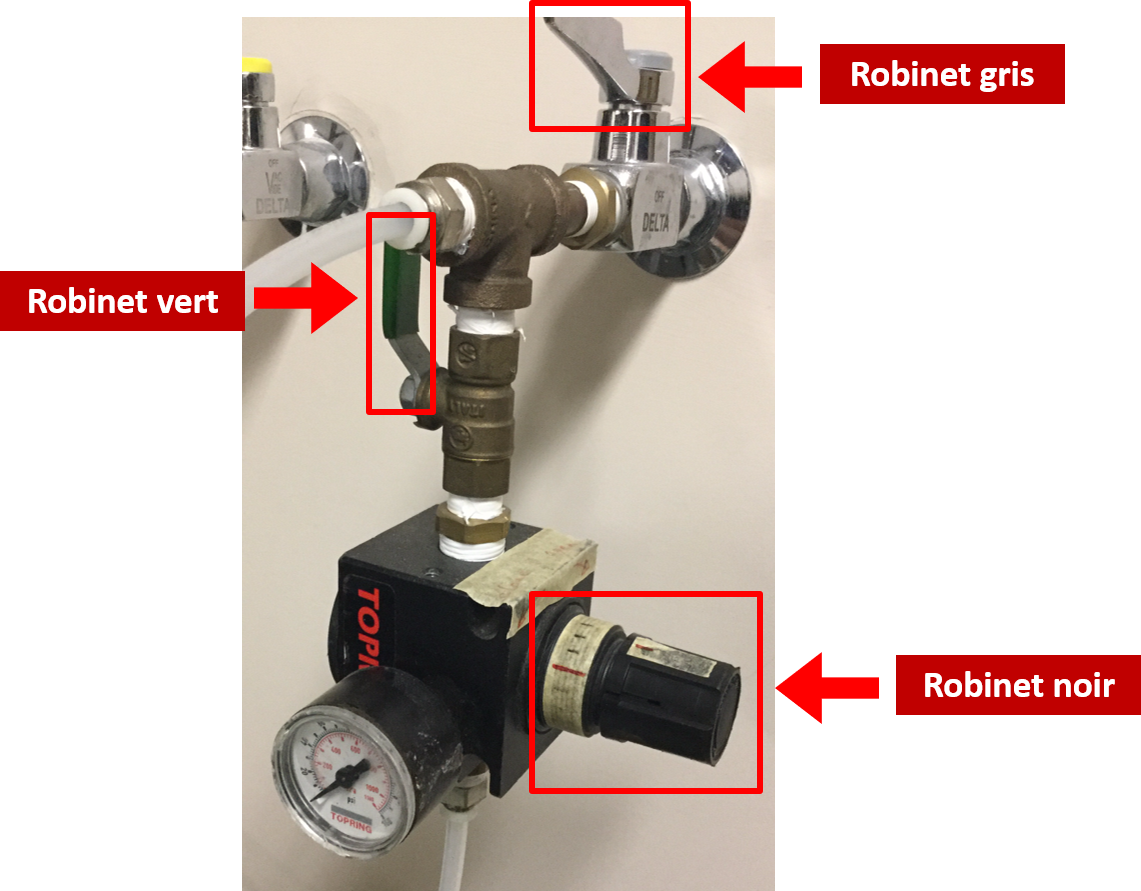
\includegraphics[width=10cm]{azote.png}
        \caption{Alimentation d'azote}
        \label{fig:azote}
        \end{figure}
        \begin{itemize}
        \item[$\bullet$] L'alimentation d'azote se trouve sur le mur juste à côté de la porte d'entrée du laboratoire.
        \item[$\bullet$] Vérifier que le \textit{robinet gris} et le \textit{robinet vert} sont positionnés comme sur la figure~\ref{fig:azote}.
        \item[$\bullet$] Tourner le \textit{robinet noir}, "suffisamment pour entendre le jet quand on approche son oreille et qu'on prête attention, mais le son ne doit pas non plus être trop fort"\footnote{François Côté, 2018}.
        \item[$\bullet$] Une fois le pourcentage d'humidité rétabli, remettre le \textit{robinet noir} à sa position initiale.
        \item[$\bullet$] Si le pourcentage d'humidité demeure élevé, il se peut qu'il y ait une fuite dans le système. Demander l'aide d'un ingénieur/physicien ou d'un superviseur.
        \end{itemize}
    \item Sur le \textit{contrôleur du RegA}, vérifier que la fréquence des impulsions (Rep. Rate) est d'environ 250-260~kHz.
    \item Sur l'\textit{oscilloscope}, vérifier que le signal a une forme semblable à ce qui est montré à la figure~\ref{fig:oscilloscope}. Les chiffres ne sont pas importants.
        \begin{figure}[H]
        \centering
        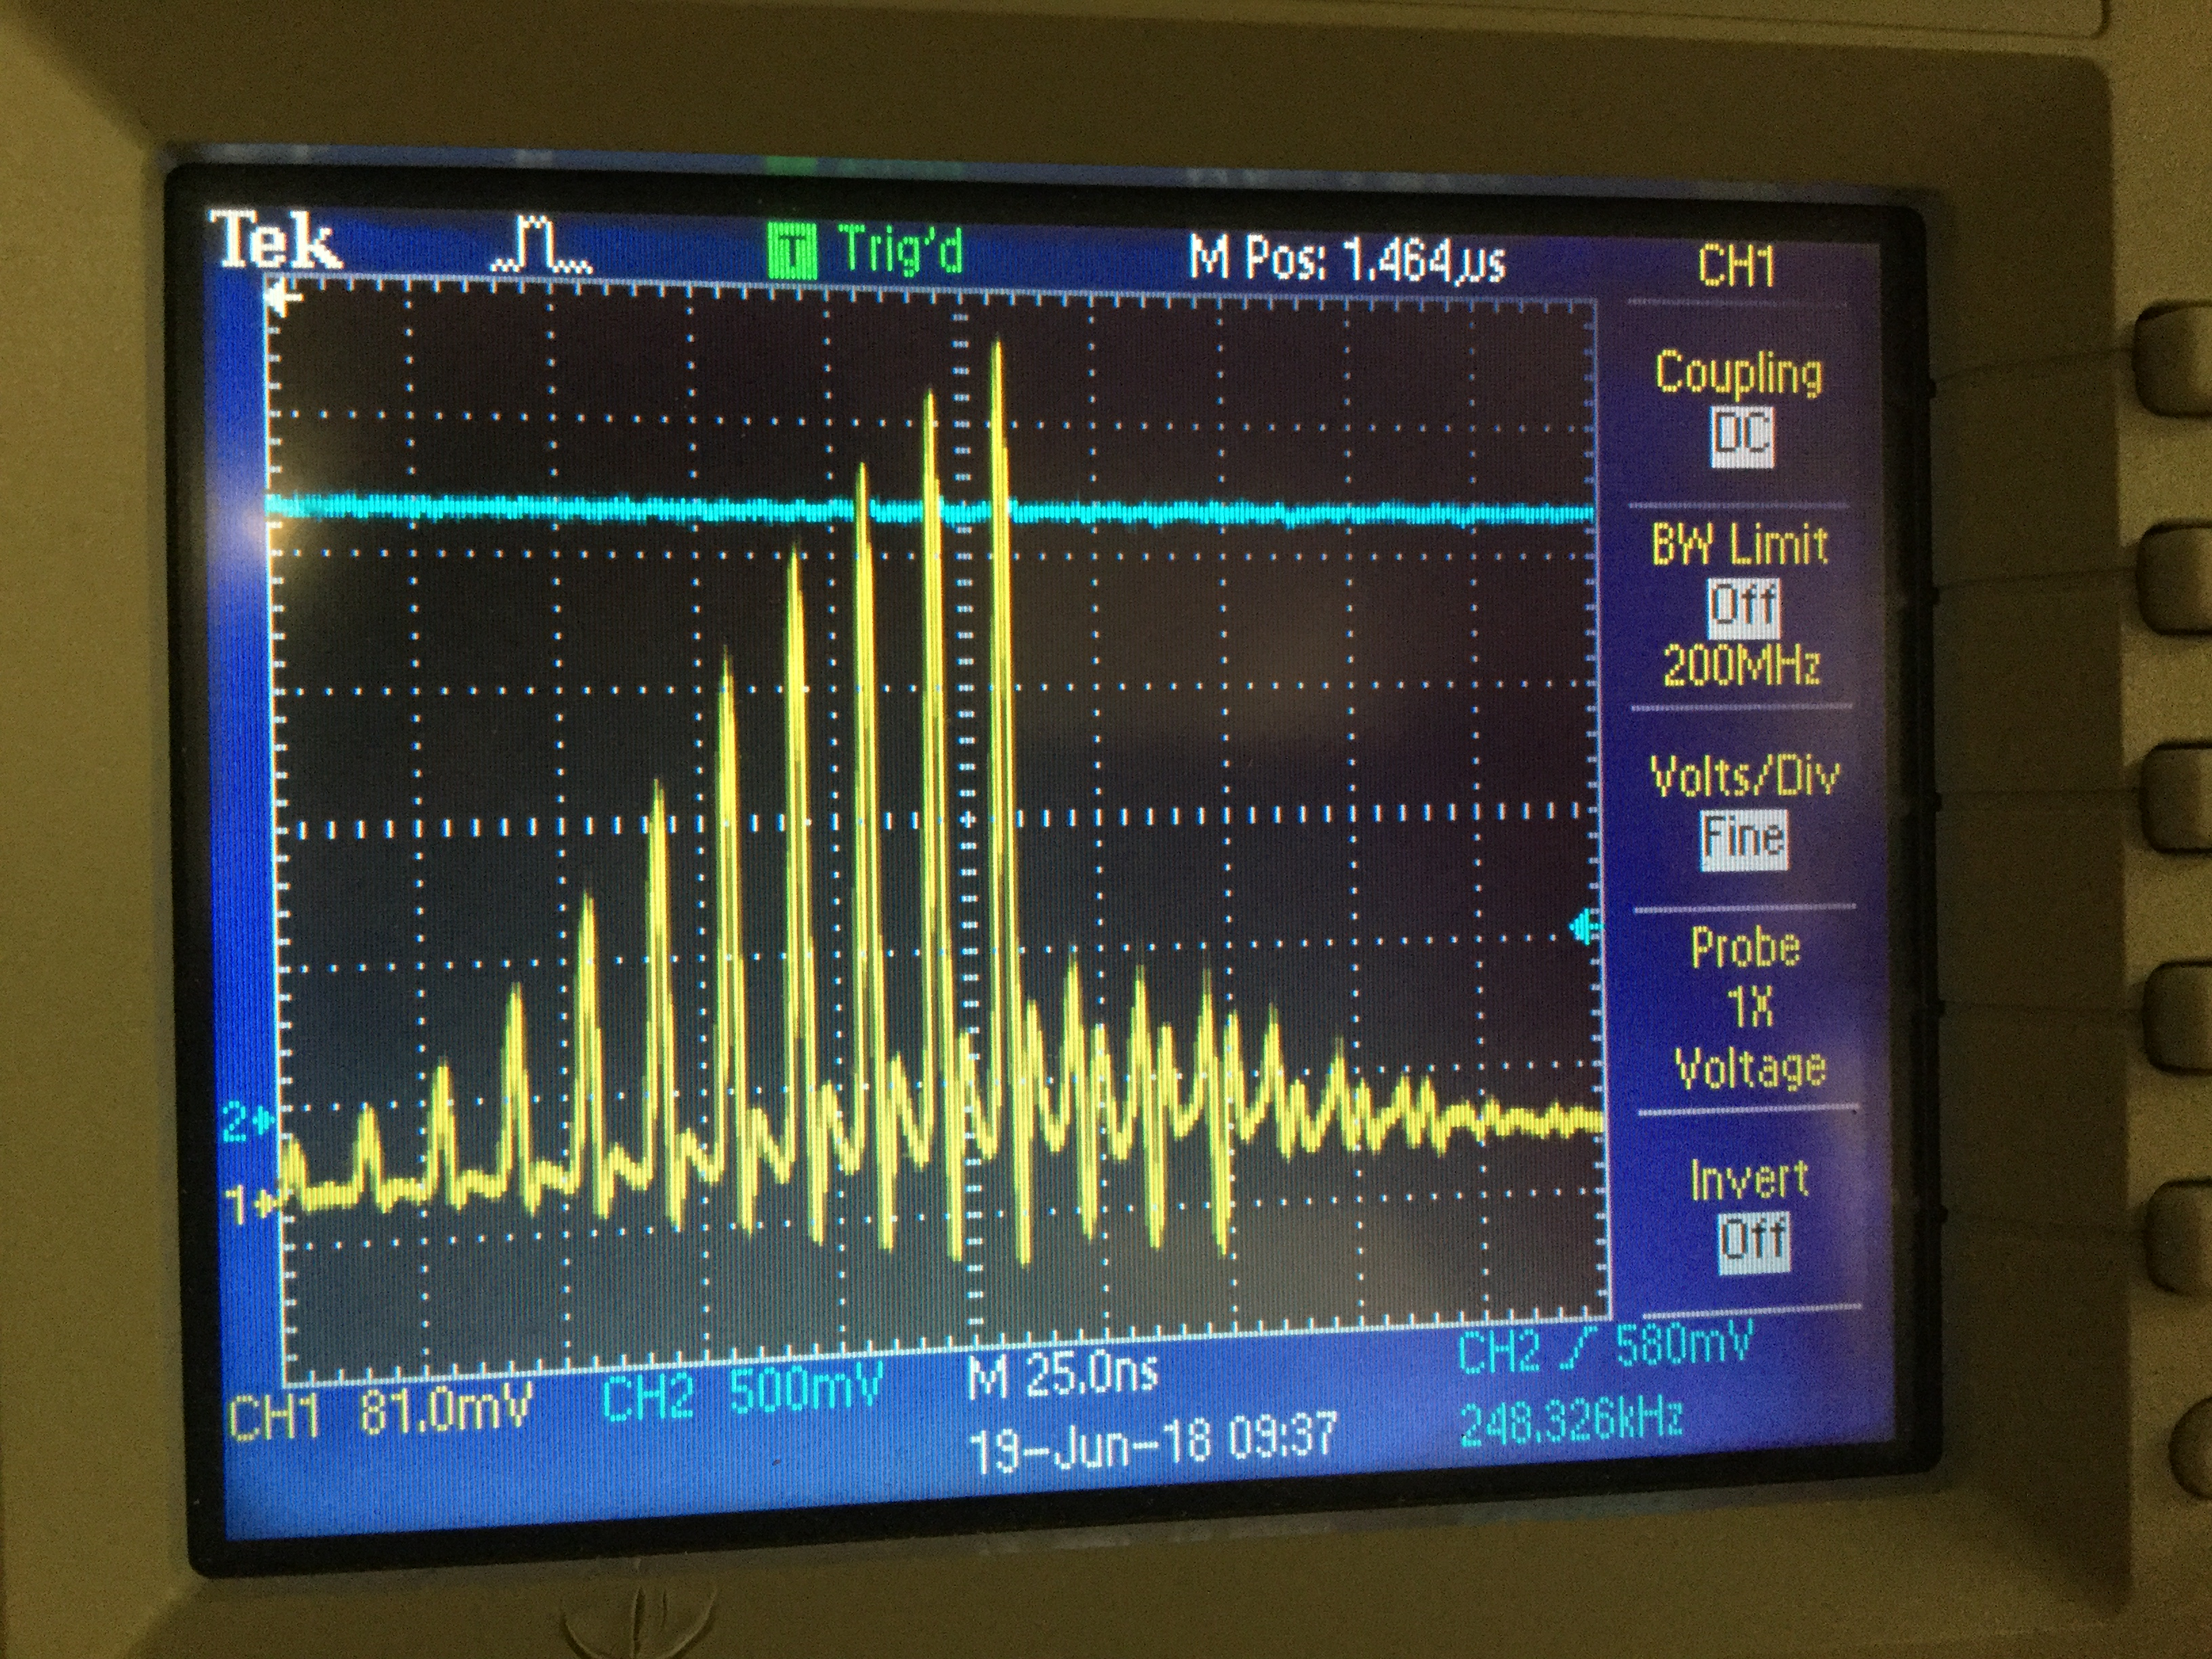
\includegraphics[width=10cm]{oscilloscope.jpg}
        \caption{Signal du laser à l'oscilloscope}
        \label{fig:oscilloscope}
        \end{figure}
    Si non, demander l'aide d'un ingénieur/physicien ou d'un superviseur.
   \item Maximiser la stabilité du signal en ajustant les \textit{switches} (voir figure~\ref{fig:controleurs}). Il ne devrait pas être nécessaire de toucher aux autres boutons des contrôleurs.
   \item A l'aide d'une carte infrarouge, vérifier que le faisceau laser a la forme d'un cercle plein à l'\textit{emplacement A} et d'un anneau à l'\textit{emplacement B} (voir figure~\ref{fig:carte}).
        \begin{figure}[H]
        \centering
        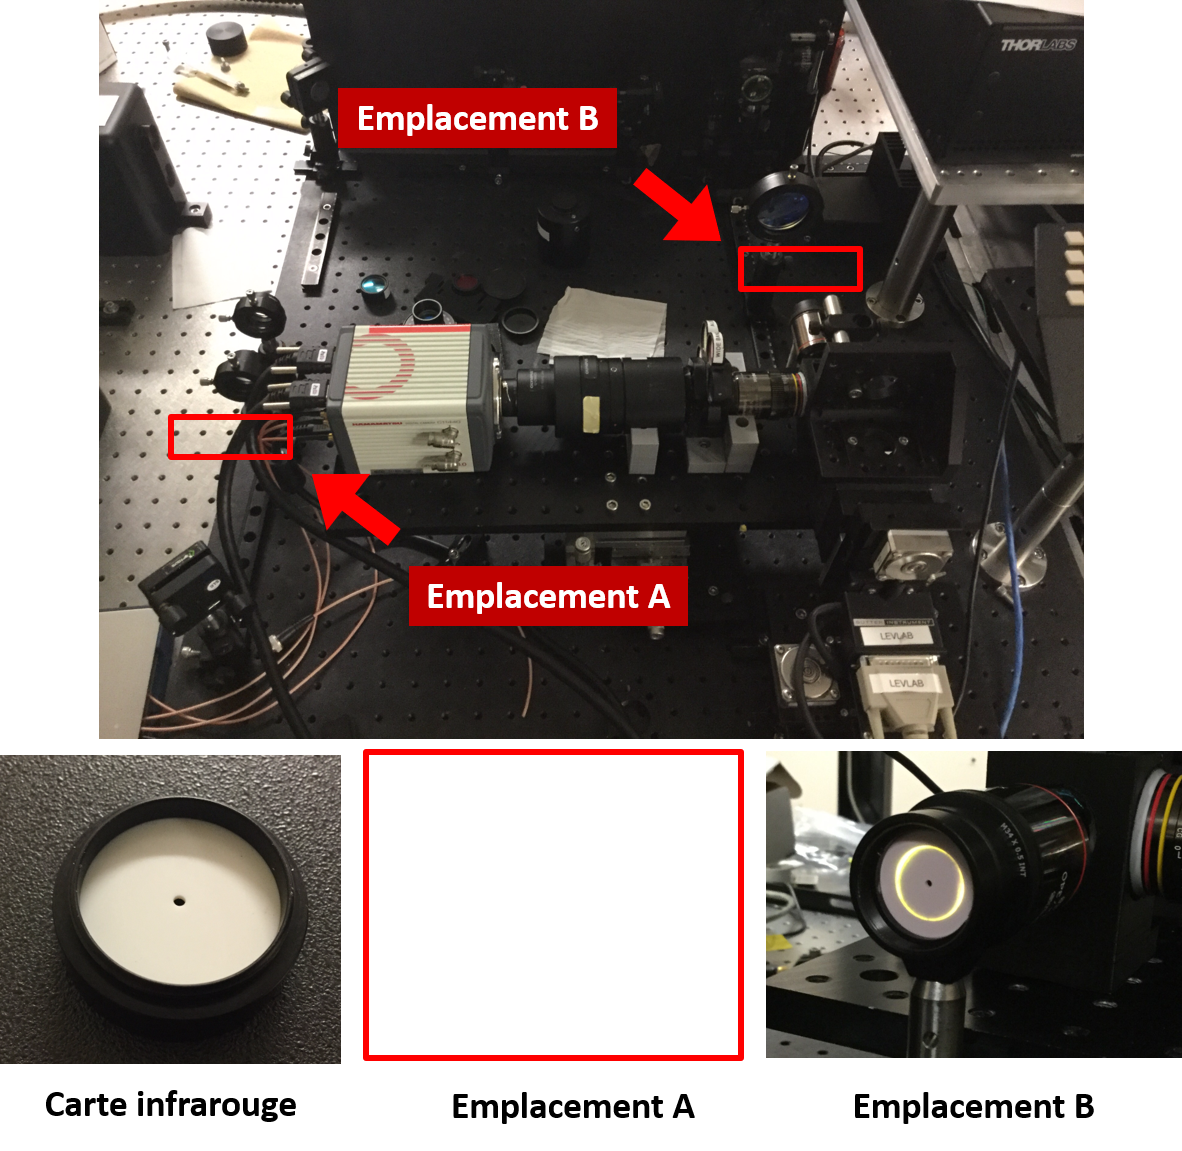
\includegraphics[width=13cm]{carte.png}
        \caption{Carte infrarouge}
        \label{fig:carte}
        \end{figure}
    Si non, il se peut que le trajet optique soit désaligné. Demander l'aide d'un ingénieur/physicien ou d'un superviseur.
   \item Sur le \textit{contrôleur du Mira}, vérifier que le laser n'a pas de composante continue (CW~=~continous wave). Sur la ligne 'Cw->' se trouvent des points '$\ldots$', un ou plusieurs carrés '$\blacksquare$' et une seule barre '|' comme montré à la figure~\ref{fig:cw}.
        \begin{figure}[H]
        \centering
        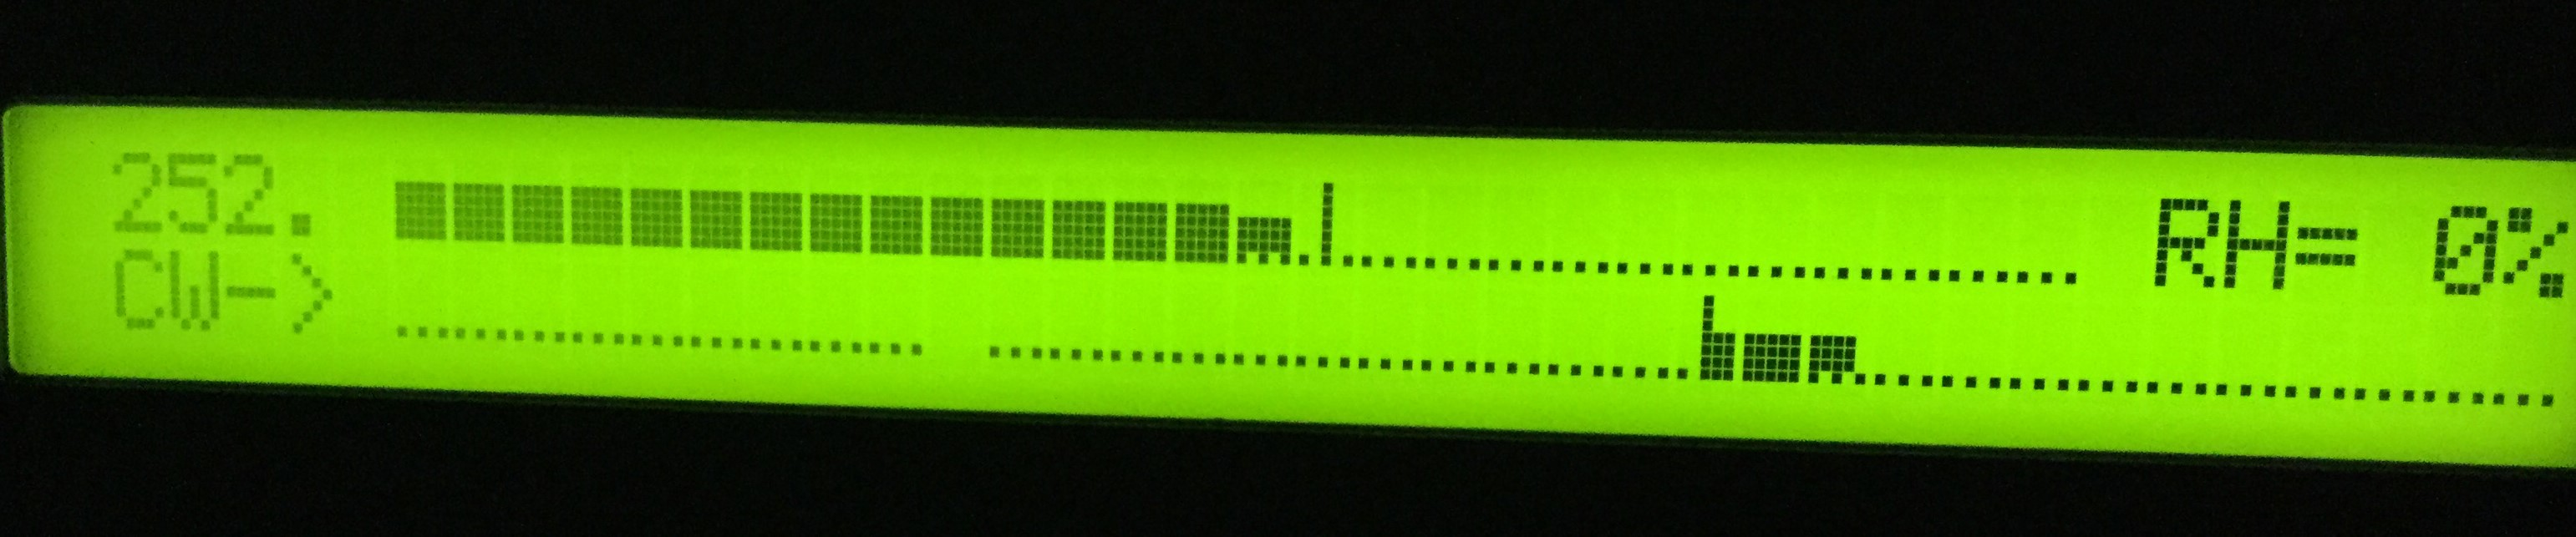
\includegraphics[width=10cm]{cw.jpg}
        \caption{Composante continue du laser}
        \label{fig:cw}
        \end{figure}
   Ajuster l'alignement afin d'avoir un seul \textit{carré} à droite de la \textit{barre}. Pour ce faire, tourner les \textit{vis} identifiées à la figure~\ref{fig:cw_vis}: celles du \textit{RegA} d'abord, puis celles du \textit{Mira} si nécessaire.
        \begin{figure}[H]
        \begin{center} \includegraphics[width=15cm]{cw_vis.png} \end{center}
        \caption{Alignement interne du \textit{RegA} et du \textit{Mira}}
        \begin{footnotesize} Le faisceau laser, pompé par le \textit{Verdi}, passe à travers le \textit{Mira} puis le \textit{RegA}. Les vis sur chacun modifient l'orientation des miroirs à l'intérieur, changeant ainsi l'alignement du laser à la sortie. \end{footnotesize}
        \label{fig:cw_vis}
        \end{figure}
\end{enumerate}